\documentclass[9pt,sans-serif]{beamer}
\usepackage{amsmath}
\usepackage{concrete}
\usetheme{Madrid}
\usecolortheme{rose}
\usefonttheme{structuresmallcapsserif}
\usepackage{bookman}

\title[Discrete Morse Theory]{Threshold-Based Graph Reconstruction Using
  Discrete Morse Theory}

\author[Sushovan Majhi]{Brittany Terese Fasy\inst{1,2}
  \and \textcolor{blue}{\textbf{Sushovan Majhi}}\inst{3}
  \and  \\ Carola Wenk\inst{4}}
\institute[]{
  \inst{1} Department of Computer Science, Montana State University
  \and
  \inst{2} Department of Mathematics, Montana State University
  \and
  \inst{3}
  \textcolor{blue}{\textbf{Department of Mathematics, Tulane University}}
  \and
  \inst{4} Department of Computer Science, Tulane University }
\date{FWCG, 2018}

\begin{document}
\frame{\titlepage}

\begin{frame}{Introduction}
  \begin{block}{Problem Statement}
    Given a (noisy) sample $S$ taken around a (hidden) embedded graph $G$, how
    one can ``\textcolor{blue}{reconstruct}'' the topology and geometry of $G$
    from $S$.
  \end{block}
  
  \begin{figure}[htb]
    \centering 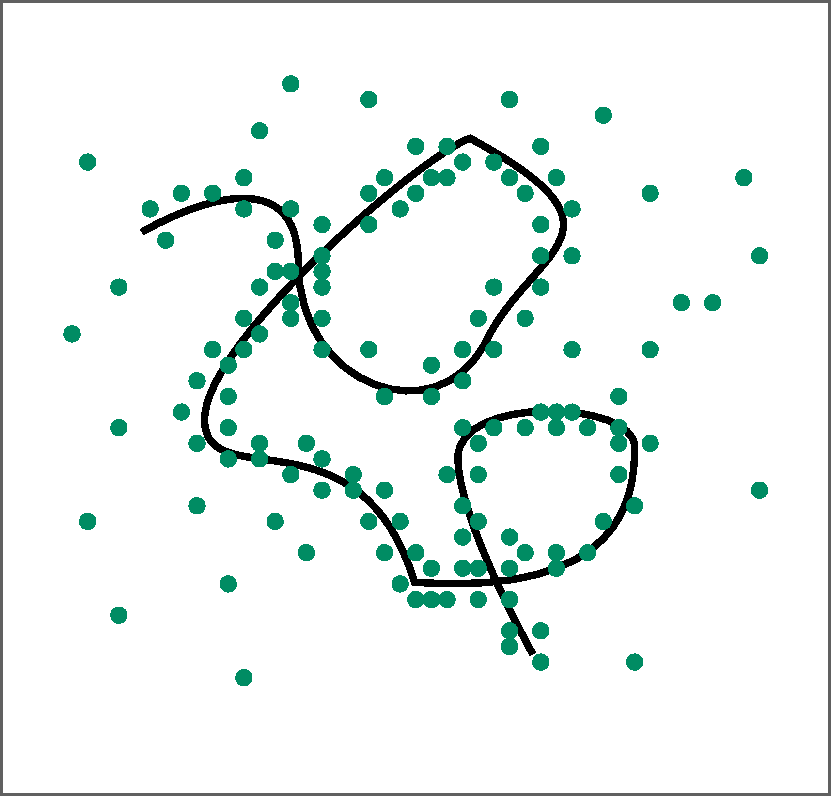
\includegraphics[scale=0.3]{sample}
    \caption{Sample around an embedded graph}
  \end{figure}
\end{frame}

\begin{frame}{Application: Map Reconstruction from GPS traces}
  \begin{figure}[htb]
    \centering 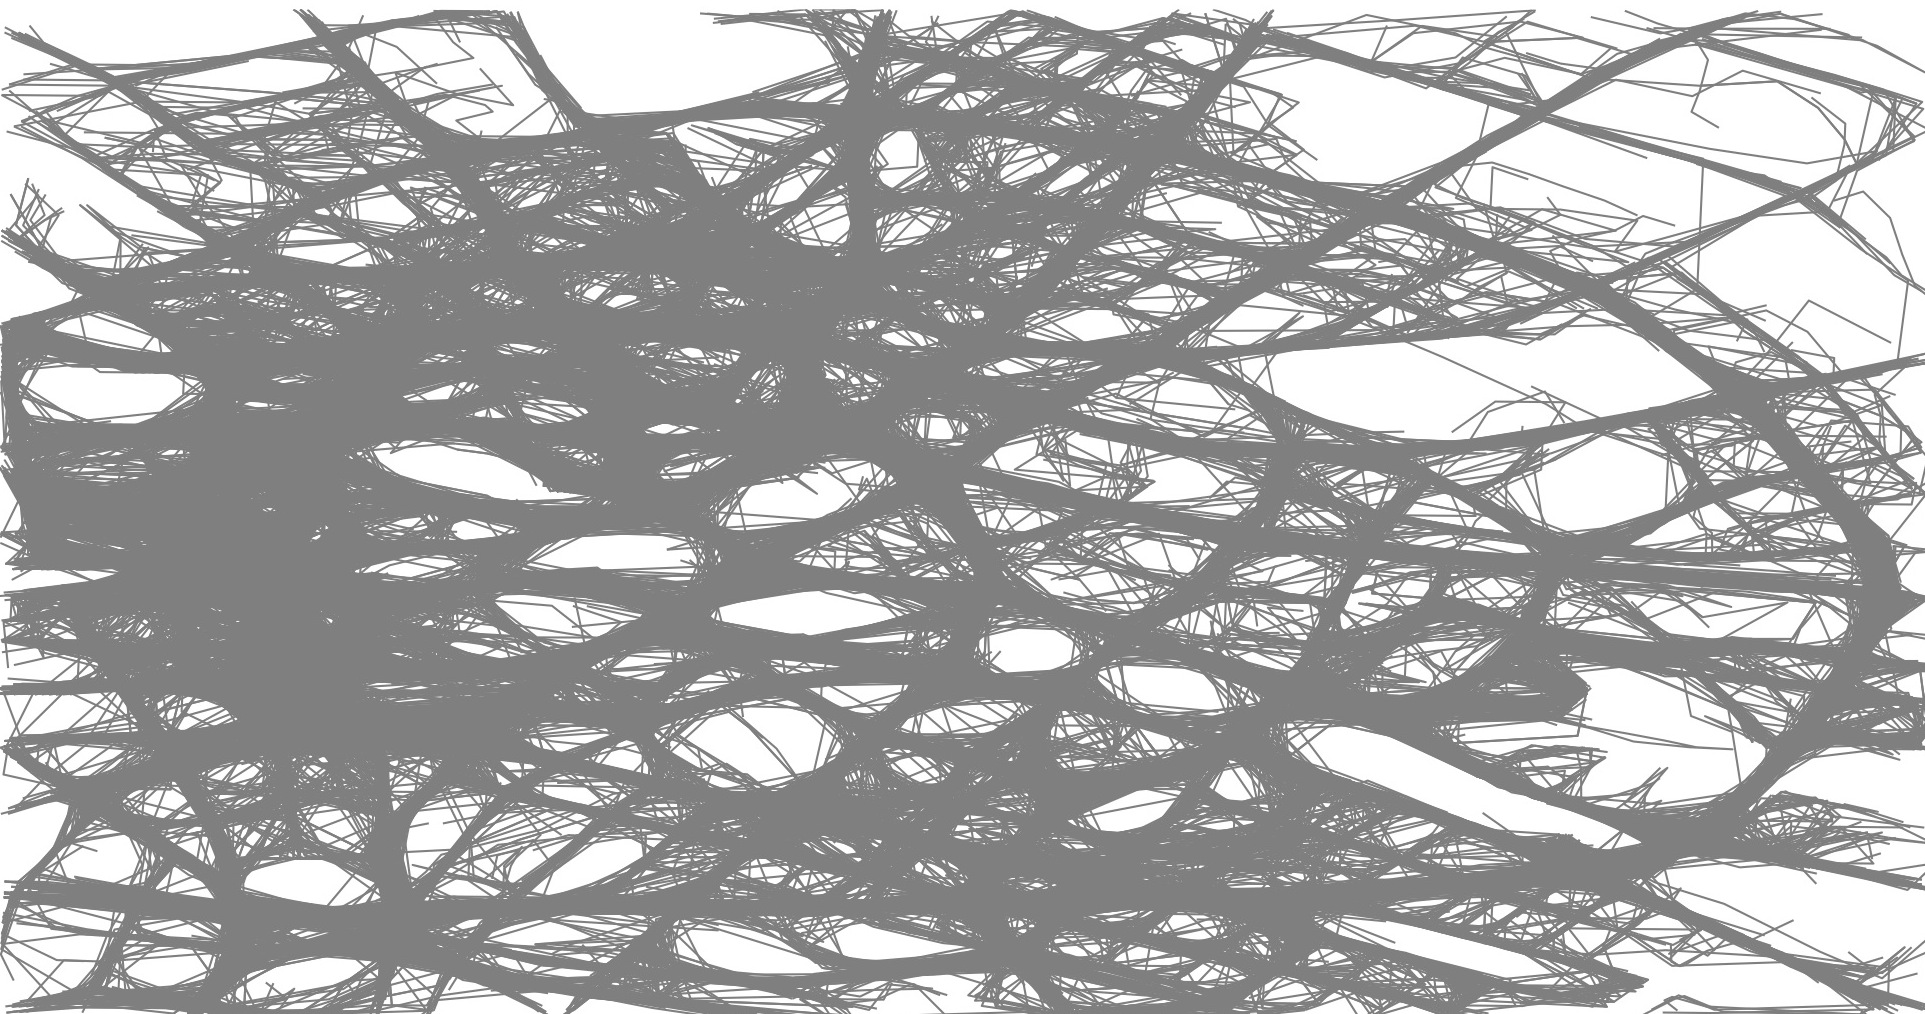
\includegraphics[scale=0.15]{Berlin}
    \caption{GPS traces of Berlin (mapconstruction.org)}
  \end{figure}
  
  \pause
  \begin{figure}[htb]
    \centering 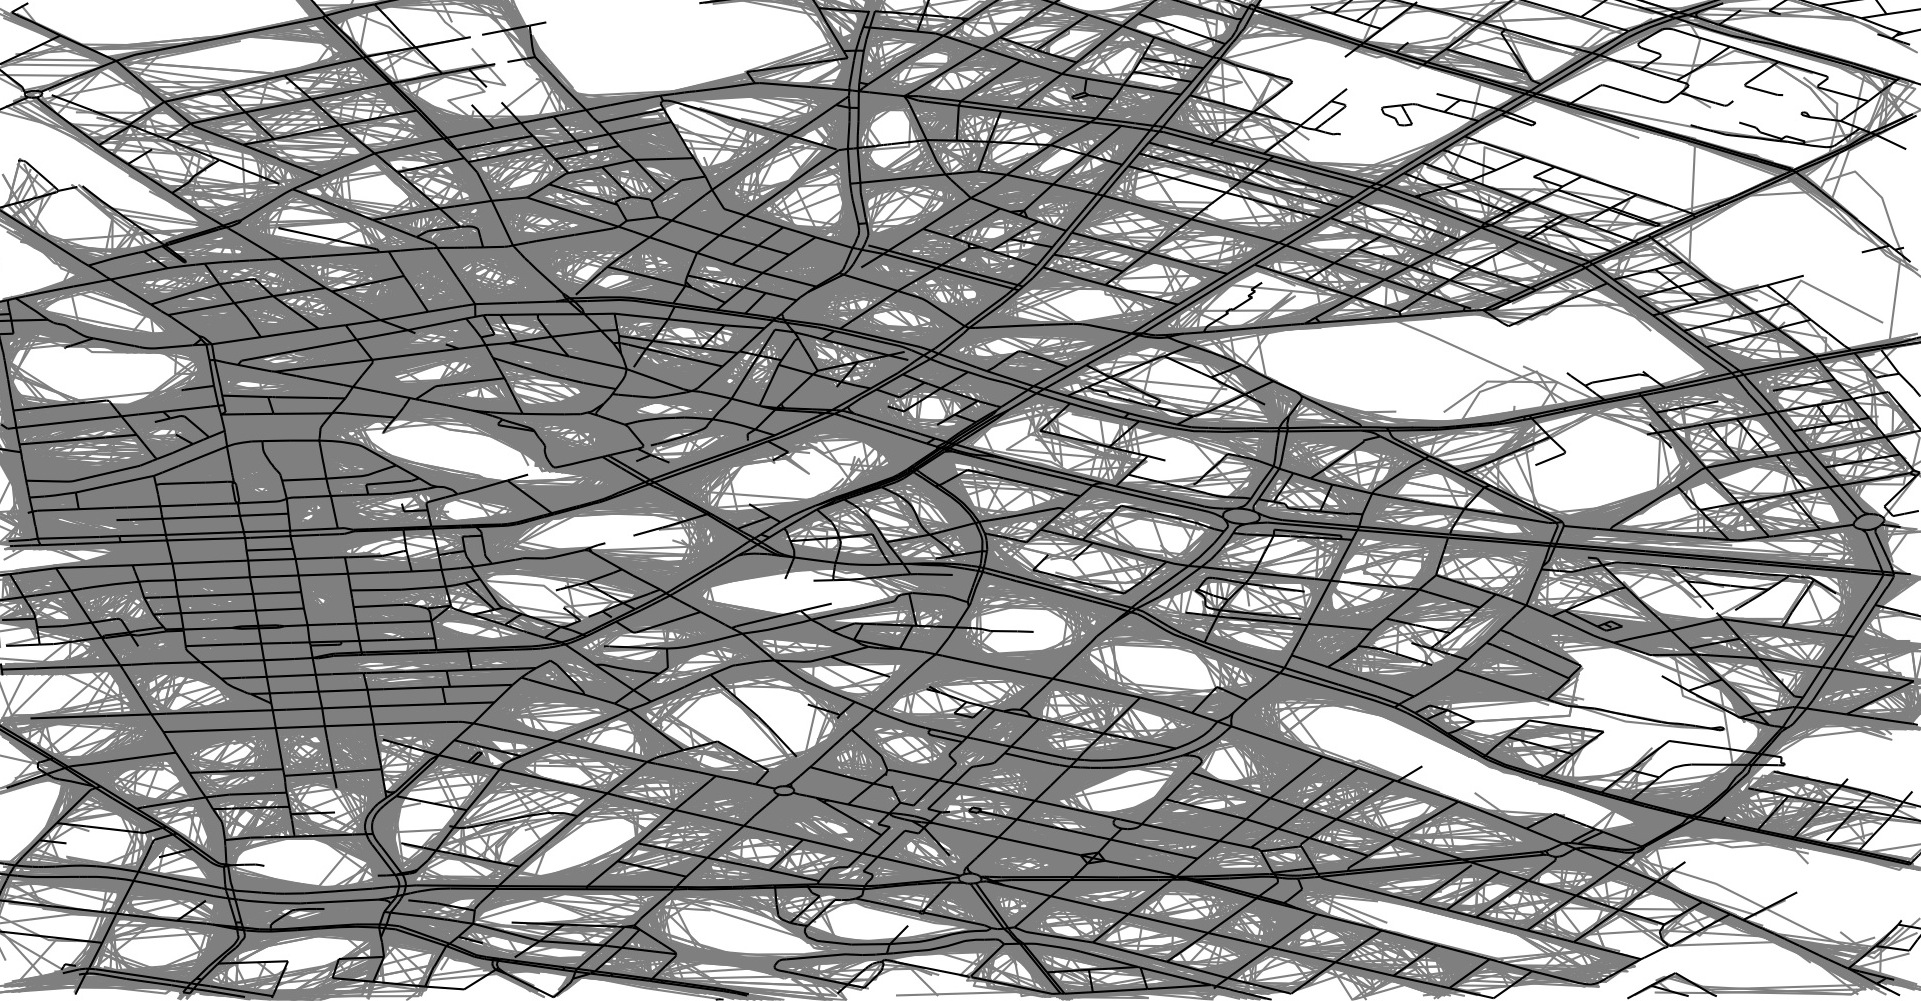
\includegraphics[scale=0.2]{Berlin_Recon}
    \caption{A reconstruction}
  \end{figure}
\end{frame}

\begin{frame}{Noise Models}
  \begin{block}{Noise Models}
    \begin{enumerate}
    \item Hausdorff noise
    \item Non-Hausdorff noise
    \end{enumerate}
  \end{block}
  
  \pause
  
  \begin{block}{What to reconstruct?}
    \begin{enumerate}
    \item Topology
      (\textcolor{blue}{same homotopy type})
    \item Geometry
      (\textcolor{blue}{small Hausdorff-distance})
    \end{enumerate}
  \end{block}
\end{frame}


\begin{frame}{Density-Based Map Construction}
  \begin{block}{Generic Density-Based Algorithm}
    Given a discretized domain $\tilde D$ and a sample $S$ around $G$.
    \begin{enumerate}
    \item Compute density $f$ of $S$ over $\tilde D$. \\
      \pause
      \begin{itemize}
        \color{blue}
      \item
        {Histogram Computation}
      \item Kernel Density Estimate
        $$K(x,y;b):=\exp\bigg(\frac{-\|x-y\|^2}{2b^2}\bigg)$$
        $$f(x)=\frac{1}{2\pi |S|b^2}\sum_{X_i\in S} K(x,X_i;b)$$
      \end{itemize}
      \pause
    \item for an appropriate threshold $t$, $f^{-1}[t,\infty)$ is considered.
      \pause
    \item heuristic pruning methods are applied this super-level set to
      approximate $G$.
    \end{enumerate}
  \end{block}
\end{frame}

\begin{frame}{Related Work}
  \begin{block}{Recent Works}
    \begin{enumerate}
    \item Choosing thresholds systematically using
      \textcolor{blue}{Persistent Homology}.
      \cite{Ahmed:2015:CTD:2820783.2820810}
      \pause
    \item Graph reconstruction by \textcolor{blue}{Discrete Morse theory}.
      \cite{dey_graph_2018_socg}
    \end{enumerate}
  \end{block}

  \pause
  
  \begin{block}{Limitations}
    \begin{enumerate}
    \item Thresholds are chosen heuristically.
    \item Theoretical guarantees on the topological/geometric correctness is not
      proved.
    \item The output is often a thick region around the hidden graph.
    \end{enumerate}
  \end{block}
\end{frame}


\begin{frame}{Assumption on the Density Function}
  \begin{block}{$(\omega,\beta_1,\beta_2,\nu)$-approximation of $G$}
    Let $\omega>0$ such that $G^\omega$ has a deformation retract onto $G$.
    \[
    f(x)\in
    \begin{cases}
      [\beta_1, \beta_1+\nu],&  x\in V^\omega \\
      [\beta_2, \beta_2+\nu],&  x\in G-V^\omega \\
      [0,\nu],& \text{ otherwise }
    \end{cases}
    \]
    $V$ denotes the set of vertices of $G$.
  \end{block}
\end{frame}

\begin{frame}{Motivation}
  \begin{figure}[htb]
    \centering 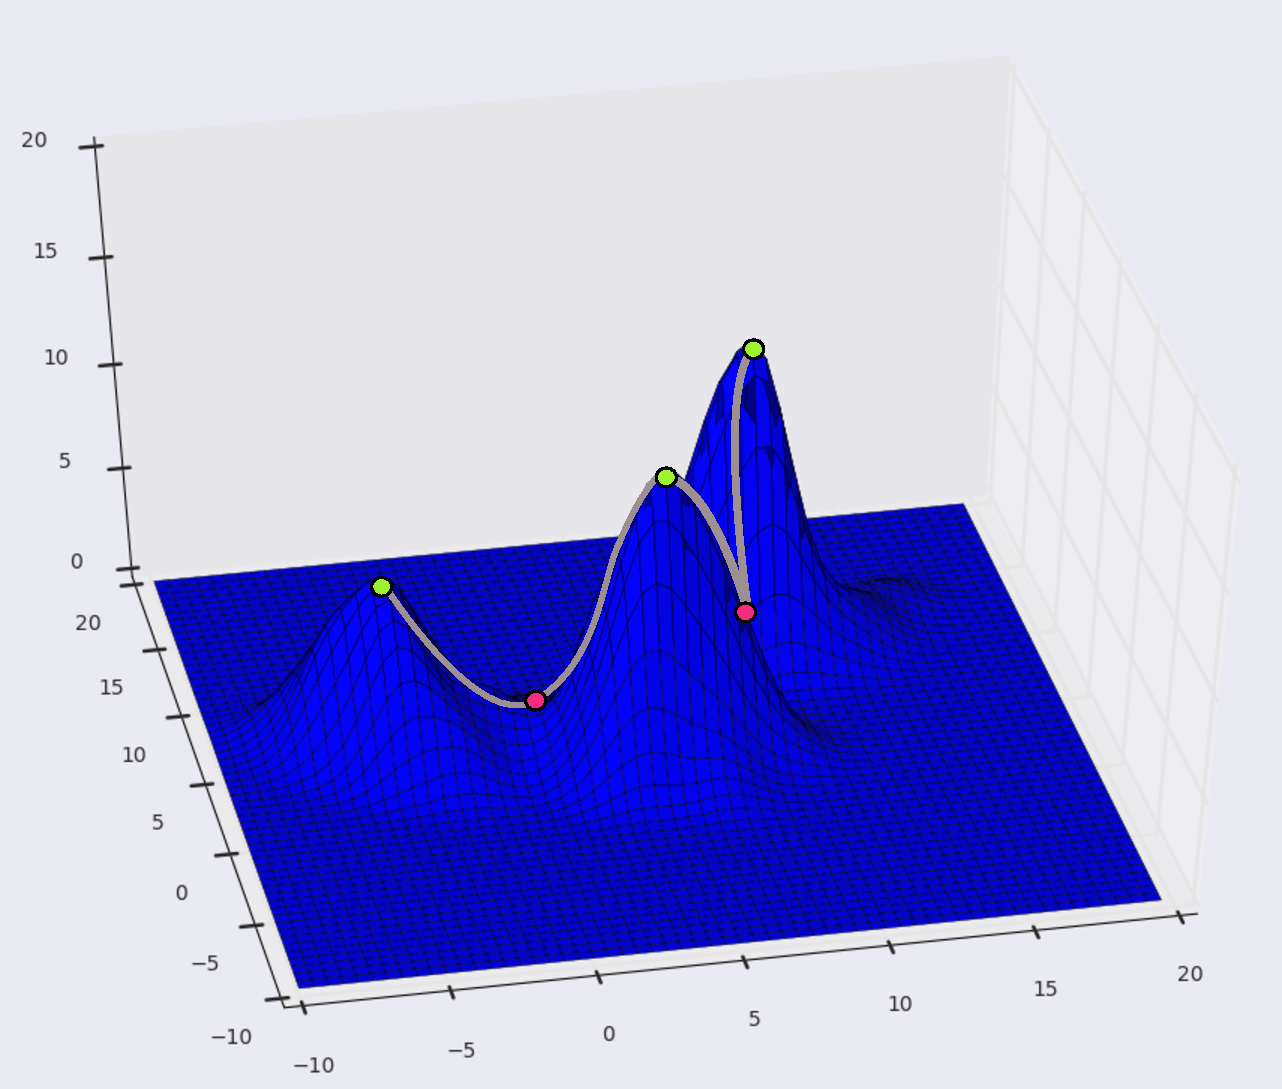
\includegraphics[scale=0.27]{ridges}
    \caption{KDE}
  \end{figure}

  \begin{block}{}
    If the samples are concentrated around a graph, then the mountain ridges on
    the graph of the density function are expected to capture it.
  \end{block}
\end{frame}


\begin{frame}{Background: Discrete Morse Theory}
 \begin{figure}[htb]
    \centering 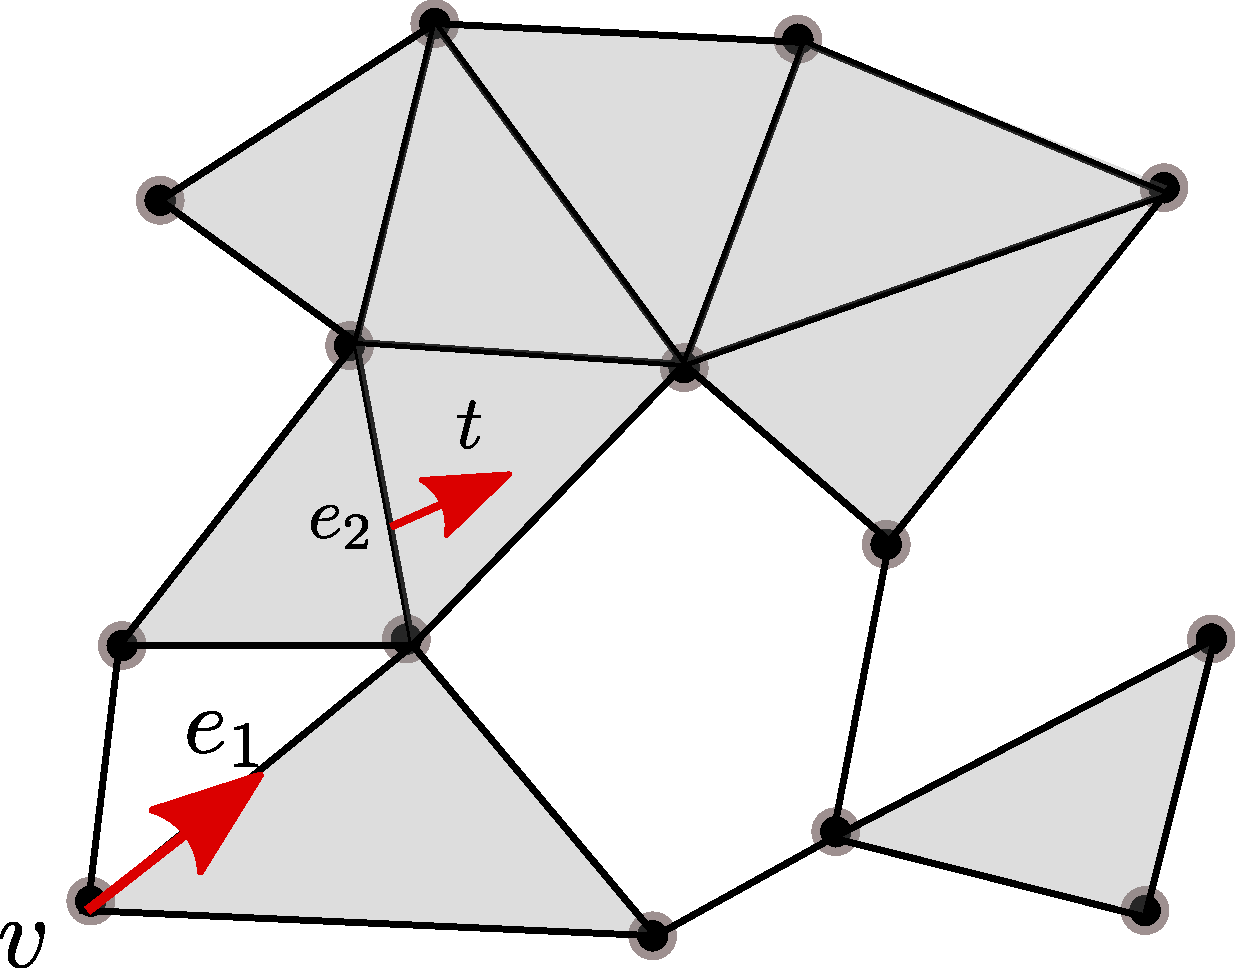
\includegraphics[scale=0.3]{vector}
    \caption{Simplicial Complex $K$ and discrete vector}
  \end{figure}

 \begin{block}{Discrete Vector}
   $(\sigma,\tau)$ is a \textcolor{blue}{discrete vector} in $K$ if
   $\sigma<\tau$ i.e. $\sigma$ is a boundary of
   $\tau$. \\ \textcolor{magenta}{$(v,e_1)$} and \textcolor{magenta}{$(e_2, t)$}
   are two discrete vectors on $K$.
 \end{block}
\end{frame}

\begin{frame}{Background: Discrete Morse Theory}
 \begin{figure}[htb]
    \centering 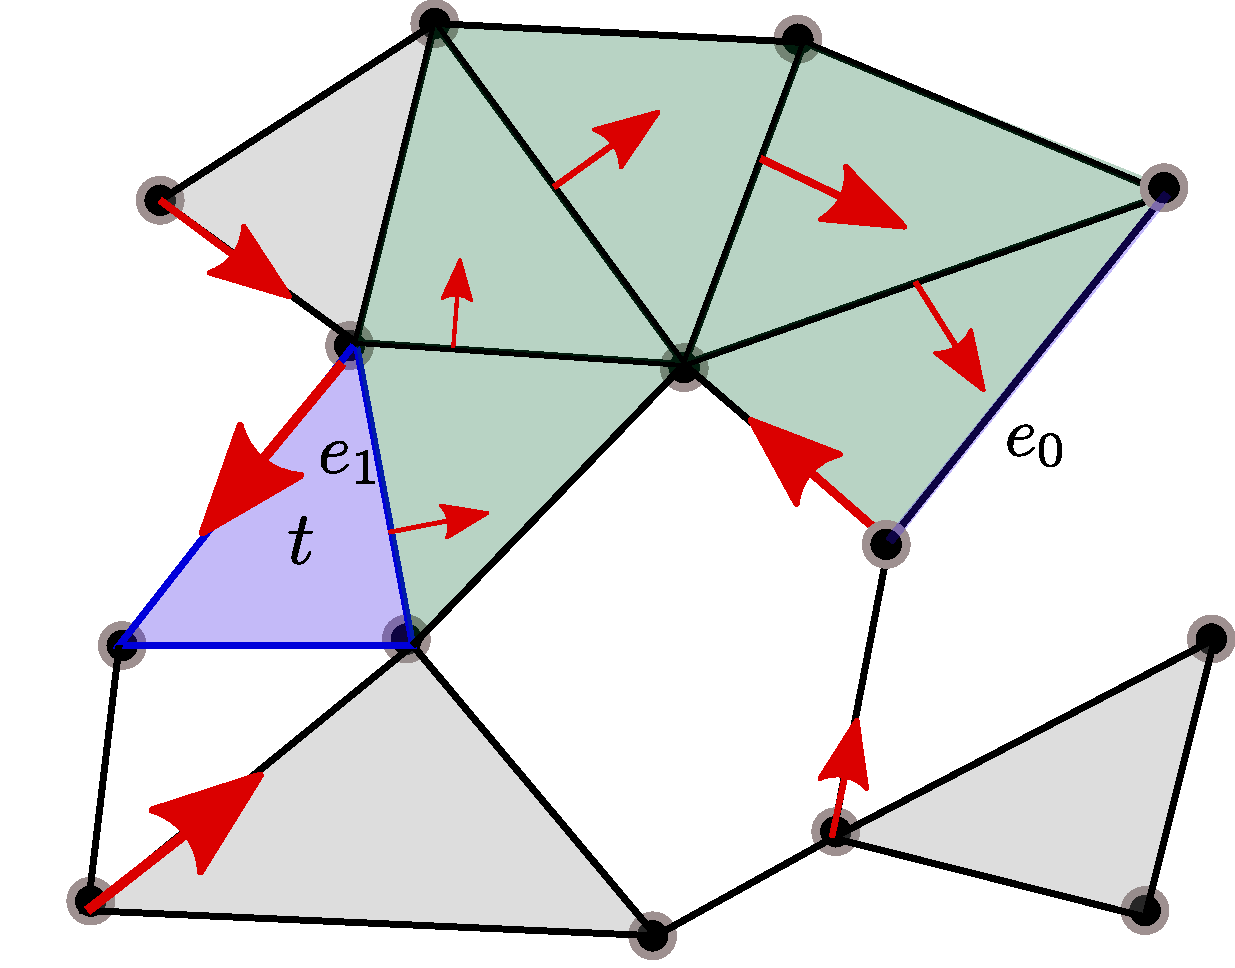
\includegraphics[scale=0.3]{vpath}
    \caption{Simplicial Complex $K$ and discrete vector}
  \end{figure}

 \begin{block}{Discrete Vector Field}
 A discrete vector field $V$ is a collection of discrete vectors such that every
 simplex of $K$ is head/tail of at most one vector.
 \end{block}
\end{frame}


\begin{frame}{Background: Discrete Morse Theory}
 \begin{figure}[htb]
    \centering 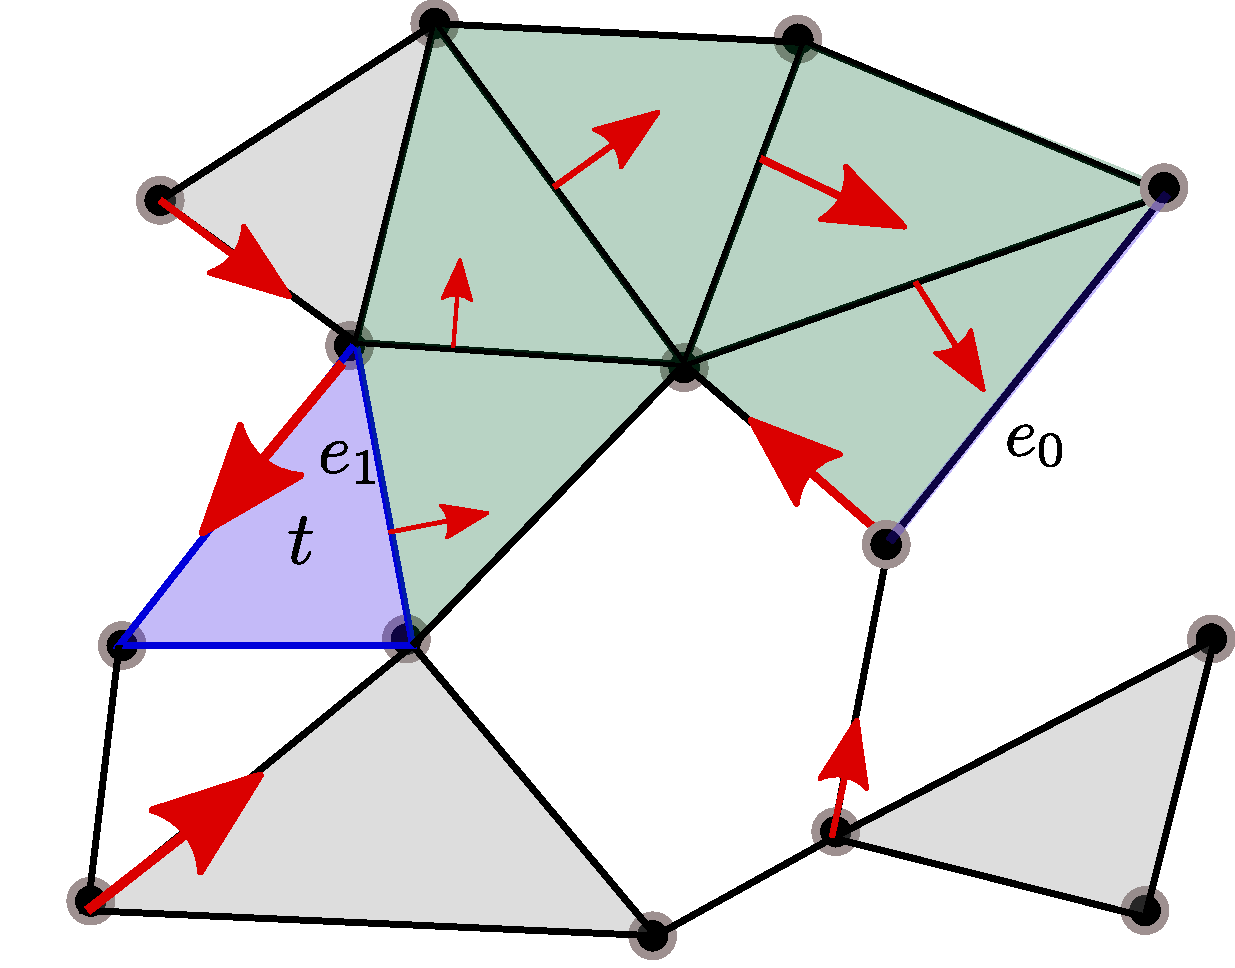
\includegraphics[scale=0.3]{vpath}
    \caption{V-path}
  \end{figure}

 \begin{block}{V-path}
   $$\sigma_0,\tau_0,\sigma_1,\tau_1,\ldots,\sigma_{l+1}$$
   where $(\sigma_i,\tau_i)$ is a vector and $\tau_i<\sigma_{i+1}$.
 \end{block}
\end{frame}

\begin{frame}{Background: Morse Cancellation}
  \begin{figure}[htb]
    \centering 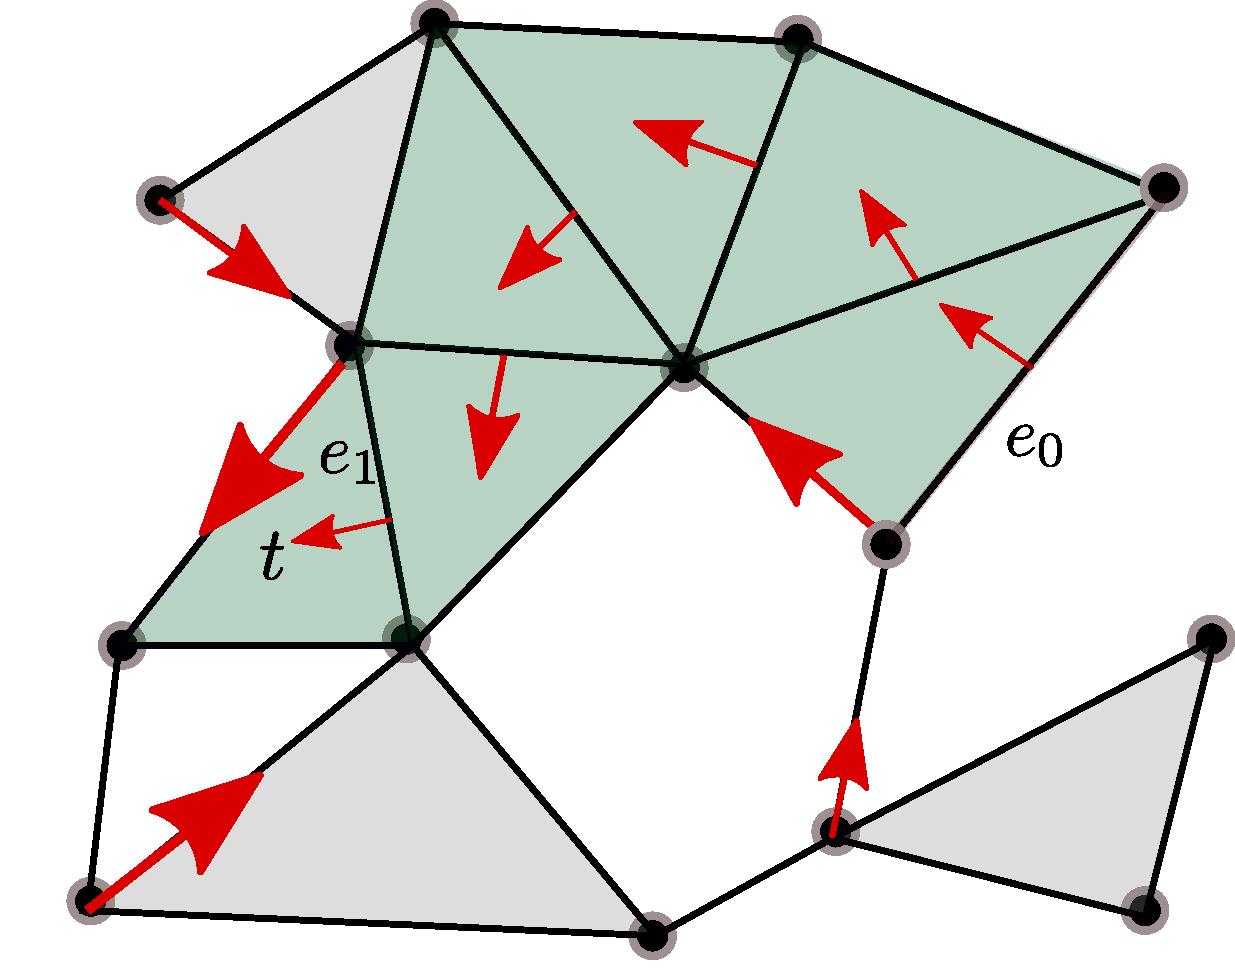
\includegraphics[scale=0.3]{cancellation}
    \caption{Morse Cancellation}
  \end{figure}

  \begin{block}{}
    Morse cancellation cancels critical points.
  \end{block}
\end{frame}

\begin{frame}{Background: Stable Manifold}
  \begin{figure}[htb]
    \centering 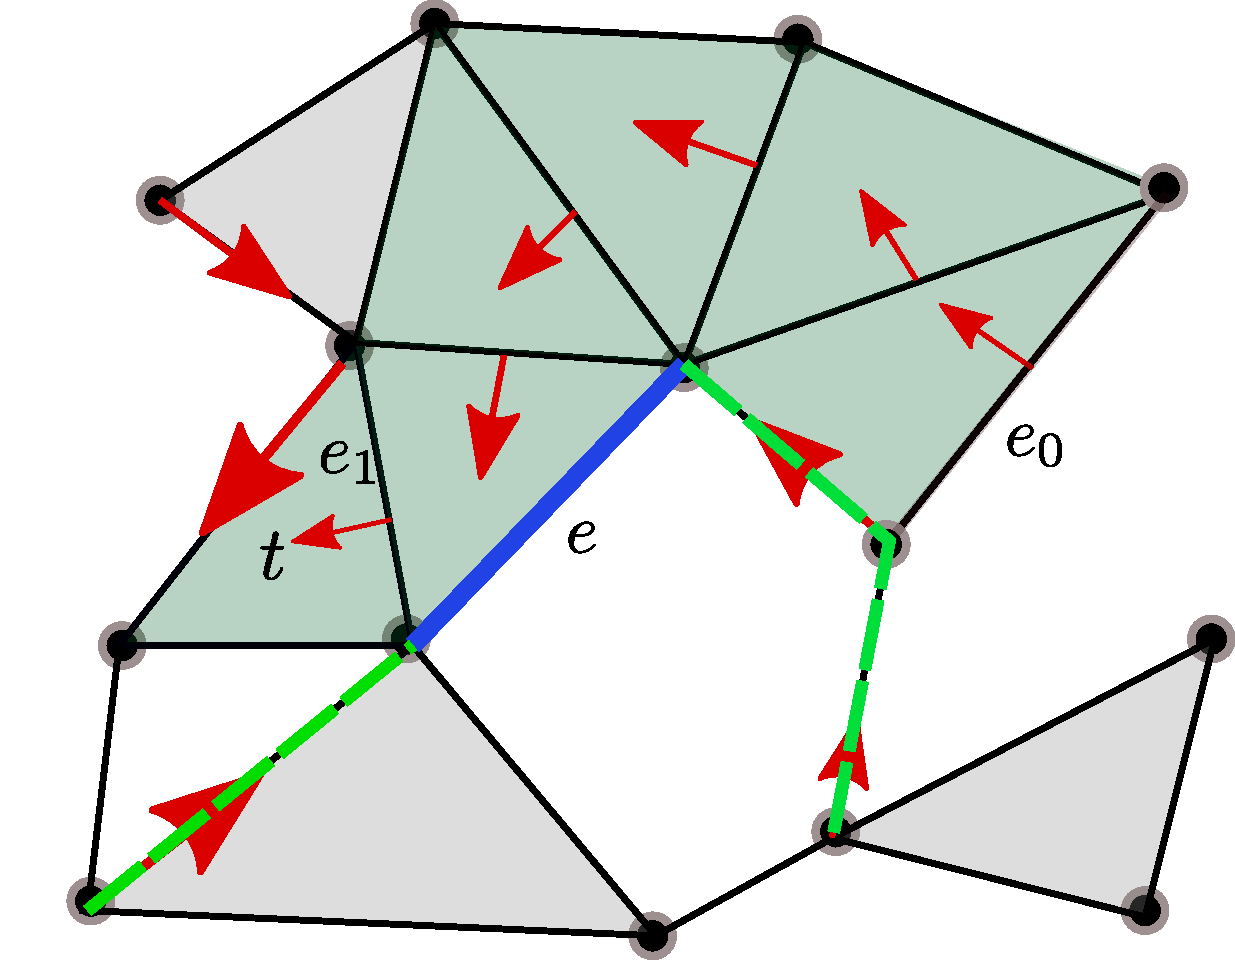
\includegraphics[scale=0.3]{stable}
    \caption{Morse Cancellation}
  \end{figure}

  \begin{block}{Stable Manifold}
    For a critical edge $e$, its \textcolor{blue}{stable manifold} is the set of
    all V-paths ending at the boundary of $e$.
  \end{block}
\end{frame}

\begin{frame}{Our Algorithm}
  Input: The discretized domain $K$, the density function $f$, the threshold
  $\delta$ \\
  Output: The reconstructed graph $\hat G$

  \pause
  
  \begin{enumerate}
  \item Initialize $V$ as the trivial vector field on $K$ and $\hat{G}=\emptyset$.

    \pause
    
  \item Run persistence on the super-level set filtration of $f$ to get the
    persistence pairs $P(K)$.

    \pause
    
  \item For each $(\sigma,\tau)\in P(K)$ with $Pers(\sigma,\tau)<\delta$ \\ Try
    to perform a Morse cancellation for the pair and update V.

    \pause
  \item For each $(v,e)\in P(K)$ and $(e,t)\in P(K)$ with $Pers(v)\geq\delta$,
    $\hat G$ = $\hat G\cup\{\text{ stable manifold of } e\}$.

    \pause
  \item   output $\hat G$
  \end{enumerate}    
\end{frame}


\begin{frame}{Our Algorithm}
  \begin{figure}[htb]
    \centering 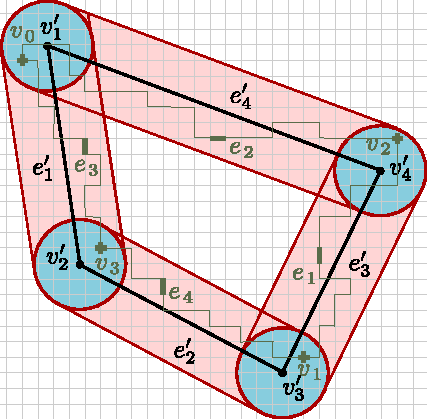
\includegraphics[scale=1]{cycle}
    \caption{Algorithm in Picture}
  \end{figure}
  
\end{frame}

\begin{frame}{Our Result}

  \begin{theorem}{}
    If $G$ is a connected, embedded planar graph in a cubical complex $K$ and
    $f$ is an $(\omega,\beta_1,\beta_2,\nu)$-approximation then the output $\hat
    G$ has the same homotopy type as $G$. Moreover, $d_H(G,\hat G)<\omega$.
  \end{theorem}
\end{frame}

  
\begin{frame}{Future Work}  
  \begin{enumerate}
  \item Extend the result to higher dimensions.
  \item What condition on the density function gives up a small Fr\'echet
    distance between the edges of the output and the edges of the graph.
  \item How to circumvent the heavy persistence computation for all nodes.
  \end{enumerate}
\end{frame}

\begin{frame}
  \centering
  \Huge{\textcolor{blue}{Thanks}} \\
  and \\
  \textcolor{magenta}{Questions?}
\end{frame}

\begin{frame}[allowframebreaks]
        \frametitle{References}
        \bibliographystyle{amsalpha}
        \bibliography{bib}
\end{frame}
\end{document}
